\documentclass[oneside,11pt,dvipsnames]{book}

\usepackage[utf8]{inputenc}
\usepackage[T1]{fontenc}
\usepackage[margin=1.5in]{geometry}
\usepackage{soul}
% \usepackage[small,compact]{titlesec} %very powerful
\usepackage[most]{tcolorbox}
% \setsecnumdepth{subsection}
% \setcounter{tocdepth}{3}
\usepackage{enumitem}
\usepackage{epigraph}
\usepackage{cite}
\usepackage{caption}
\captionsetup{font=small}
\usepackage{graphicx}
\usepackage{pdfpages}
\usepackage{hyperref}
\usepackage{wrapfig}
\setlength\intextsep{0pt} % remove extra space above and below in-line float
\usepackage{hyperref}
\hypersetup{
  colorlinks,
  citecolor=black,
  filecolor=black,
  linkcolor=blue,
  urlcolor=blue,
}
\usepackage{booktabs}


\usepackage{tikz}
\usetikzlibrary{calc}
\usepackage{xcolor}

\usepackage{anyfontsize}
\usepackage{sectsty}

\usepackage[makeroom]{cancel}

\usepackage[linesnumbered,ruled,vlined]{algorithm2e}

\SetAlgoCaptionSeparator{.}
\SetAlCapFnt{\footnotesize\rm}
\SetAlCapNameFnt{\footnotesize\rm}






\newcommand{\functiontextformat}[1]{\textrm{\texttt{#1}}}

% \newtoggle{usecomment}
% \settoggle{usecomment}{true}

% \newcommand{\tcomment}[1]{\iftoggle{usecomment}{#1}{}}
% \newcommand{\tvn}[1]{\iftoggle{usecomment}{{\color{red}{[TVN]: #1}}}{}}

% \newcommand{\mbd}[1]{\iftoggle{usecomment}{{\color{magenta}{[MBD]: #1}}}{}}
% \newcommand{\matt}[1]{\iftoggle{usecomment}{{\color{magenta}{[MBD]: #1}}}{}}

% \newcommand{\hd}[1]{\iftoggle{usecomment}{{\color{blue}{[HD]: #1}}}{}}

% \newcommand{\mynew}[1]{\iftoggle{usecomment}{{\color{red}{[NEW]: #1}}}{}}


%\newcommand{\ignore}[1]{}





\newtcolorbox{mybox}{
  enhanced,
  boxrule=0pt,frame hidden,
  borderline west={2pt}{0pt}{green!75!black},
  colback=green!10!white,
  sharp corners
}

\newenvironment{commentbox}[1][]{
  \small
  \begin{mybox}
    {\small \textbf{#1}}
  }{
  \end{mybox}
}

\newtcolorbox{mydomesticbox}{
  enhanced,
  boxrule=0pt,frame hidden,
  borderline west={2pt}{0pt}{red!75!black},
  colback=blue!10!white,
  sharp corners
}

\newenvironment{domesticbox}[1][]{
  \small
  \begin{mydomesticbox}
    {\small \textbf{#1}}
  }{
  \end{mydomesticbox}
}

% for captions
\def\Section{\S}
\renewcommand{\figurename}{Fig.}
\renewcommand{\tablename}{Tab.}
\renewcommand{\algorithmcfname}{Alg.}


% for cross references
% \renewcommand{\algorithmcflinename}{L.}
\renewcommand{\algorithmautorefname}{Alg.}
\renewcommand{\figureautorefname}{Fig.}
\renewcommand{\tableautorefname}{Tab.}
\renewcommand{\equationautorefname}{Eq.}
\renewcommand{\chapterautorefname}{\S\@gobble}
\renewcommand{\sectionautorefname}{\S\@gobble}
\renewcommand{\subsectionautorefname}{\S\@gobble}
\renewcommand{\appendixautorefname}{\S\@gobble}



\newcommand{\nnproofgen}{\texttt{APTPgen}}
\newcommand{\nnproofcheck}{\texttt{APTPcheck}}
\newcommand{\nnproofchecker}{\texttt{APTPchecker}}
\newcommand{\nnproofformat}{\texttt{APTP}}
%\newcommand{\tool}{\texttt{NNProofChecker}}
\newcommand{\veristable}{\texttt{VeriStable}}
\newcommand{\crown}{\texttt{$\alpha\beta$-CROWN}}
\newcommand{\nnenum}{\texttt{nnenum}}
\newcommand{\marabou}{\texttt{Marabou}}
\newcommand{\eran}{\texttt{ERAN}}
\newcommand{\reluplex}{\texttt{Reluplex}}
\newcommand{\reluval}{\texttt{Reluval}}
\newcommand{\neurify}{\texttt{Neurify}}
\newcommand{\nnv}{\texttt{NNV}}
\newcommand{\ovalnnv}{\texttt{OVAL}}
\newcommand{\dnnv}{\texttt{DNNV}}
\newcommand{\verinet}{\texttt{VeriNet}}
\newcommand{\mnbab}{\texttt{MN-BaB}}
% \newcommand{\vnncomp}{VNN-COMP'23}
\newcommand{\planet}{\texttt{Planet}}
\newcommand{\dd}{\texttt{BaB$_{\text{NV}}$}}
\newcommand{\neuralsat}{\texttt{NeuralSAT}}
\newcommand{\mipverify}{\texttt{MIPVerify}}
\newcommand{\crowndefault}{\texttt{$\alpha\beta$-CROWN} (default)}

\makeatletter
\makeatother

\newcommand{\mycomment}[3][\color{blue}]{{#1{{#2}: {#3}}}}
\newcommand{\tvn}[1]{\mycomment{TVN}{#1}}{}
\newcommand{\didi}[1]{\mycomment{Didier}{#1}}{}
\newcommand{\tl}[1]{\mycomment{ThanhLe}{#1}}{}
\newcommand{\red}[1]{{\color{red}{#1}}}
\newcommand{\xz}[1]{\mycomment{Xiaokuan}{[#1]}}{}


\begin{document}

\pagestyle{empty}
\begin{tikzpicture}[overlay,remember picture]

    % Background color
    \fill[
    black!2]
    (current page.south west) rectangle (current page.north east);
    
    % Rectangles
    \shade[
    left color=Dandelion, 
    right color=Dandelion!40,
    transform canvas ={rotate around ={45:($(current page.north west)+(0,-6)$)}}] 
    ($(current page.north west)+(0,-6)$) rectangle ++(9,1.5);
    
    \shade[
    left color=lightgray,
    right color=lightgray!50,
    rounded corners=0.75cm,
    transform canvas ={rotate around ={45:($(current page.north west)+(.5,-10)$)}}]
    ($(current page.north west)+(0.5,-10)$) rectangle ++(15,1.5);
    
    \shade[
    left color=lightgray,
    rounded corners=0.3cm,
    transform canvas ={rotate around ={45:($(current page.north west)+(.5,-10)$)}}] ($(current page.north west)+(1.5,-9.55)$) rectangle ++(7,.6);
    
    \shade[
    left color=orange!80,
    right color=orange!60,
    rounded corners=0.4cm,
    transform canvas ={rotate around ={45:($(current page.north)+(-1.5,-3)$)}}]
    ($(current page.north)+(-1.5,-3)$) rectangle ++(9,0.8);
    
    \shade[
    left color=red!80,
    right color=red!80,
    rounded corners=0.9cm,
    transform canvas ={rotate around ={45:($(current page.north)+(-3,-8)$)}}] ($(current page.north)+(-3,-8)$) rectangle ++(15,1.8);
    
    \shade[
    left color=orange,
    right color=Dandelion,
    rounded corners=0.9cm,
    transform canvas ={rotate around ={45:($(current page.north west)+(4,-15.5)$)}}]
    ($(current page.north west)+(4,-15.5)$) rectangle ++(30,1.8);
    
    \shade[
    left color=RoyalBlue,
    right color=Emerald,
    rounded corners=0.75cm,
    transform canvas ={rotate around ={45:($(current page.north west)+(13,-10)$)}}]
    ($(current page.north west)+(13,-10)$) rectangle ++(15,1.5);
    
    \shade[
    left color=ForestGreen,
    rounded corners=0.3cm,
    transform canvas ={rotate around ={45:($(current page.north west)+(18,-8)$)}}]
    ($(current page.north west)+(18,-8)$) rectangle ++(15,0.6);
    
    \shade[
    left color=ForestGreen,
    rounded corners=0.4cm,
    transform canvas ={rotate around ={45:($(current page.north west)+(19,-5.65)$)}}]
    ($(current page.north west)+(19,-5.65)$) rectangle ++(15,0.8);
    
    \shade[
    left color=OrangeRed,
    right color=red!80,
    rounded corners=0.6cm,
    transform canvas ={rotate around ={45:($(current page.north west)+(20,-9)$)}}] 
    ($(current page.north west)+(20,-9)$) rectangle ++(14,1.2);
    
 
    
    % Title
    \node[align=center] at ($(current page.center)+(0,-5)$) 
    {
        {\fontsize{24}{24} \selectfont {{Engineering A Verifier}}} \\[0.15in]
        {\fontsize{24}{24} \selectfont {{for Deep Neural Networks}}} \\[1in]    
        %{\fontsize{18}{18} \selectfont {{A Handbook for International Students}}} \\[1.in]

    {\fontsize{14}{19.2} \selectfont \textcolor{ForestGreen}{ \bf ThanhVu (Vu) Nguyen}}\\[0.1in]
    \today{} (latest version available on  \href{https://github.com/nguyenthanhvuh/phd-cs-us}{Github})
    };
    \end{tikzpicture}

    
\chapter*{Preface}
Having been involved in PhD admission committees for many years, I've realized that many \textbf{international} students, especially those in smaller countries or less well-known universities, lack a clear understanding of
the Computer Science PhD admission process at US universities. This confusion not only
discourages students from applying but also creates the perception that
getting admitted to a CS PhD program in the US is difficult compared to other countries.

% though \emph{very} top schools could be very selective, e.g., see the \href{https://da-data.blogspot.com/2015/03/reflecting-on-cs-graduate-admissions.html}{admission process} at CMU
So I want to share some details about the admission process and advice for those who are interested in applying for a \textbf{PhD in Computer Science in the US}.
Originally, this document was intended for international students, but I have expanded it to include information that might also be useful for \emph{US domestic students}.
Moreover, while this is primarily intended for students interested in CS, it might be relevant to students from various STEM (Science, Technologies, Engineering, and Mathematics) disciplines.
Furthermore, although many examples are specifics for schools that I and other contributors of this document know about, the information should be generalizable to other R1\footnote{An \href{https://en.wikipedia.org/wiki/List_of_research_universities_in_the_United_States}{R1 institution} in the US is a research-intensive university with a high level of research activity across various disciplines. Currently, 146 (out of 4000) US universities are classified as R1.} institutions in the US.

This information can also help \textbf{US faculty and admission committee} gain a better understanding of international students and their cultural differences.  By recognizing and leveraging these differences, CS programs in the US can attract larger and more competitive application pools from international students.

I wish you the best of luck. Happy school hunting!

\begin{mybox}
This document will be updated regularly to reflect the latest information and updates in the admission process. Its latest version is available at

\begin{center}
  \href{https://nguyenthanhvuh.github.io/phd-cs-us/demystify.pdf}{nguyenthanhvuh.github.io/phd-cs-us/demystify.pdf},
\end{center}

\noindent and its \LaTeX{} source is also on \href{https://github.com/nguyenthanhvuh/phd-cs-us}{GitHub}. If you have questions or comments, feel free to create new \href{https://github.com/nguyenthanhvuh/phd-cs-us/issues}{GitHub issues} or \href{https://github.com/nguyenthanhvuh/phd-cs-us/discussions}{discussions}.

\end{mybox}

\newpage
\tableofcontents

\chapter{Basic of Neural Network}\label{sec:basic}

A \emph{neural network} (\textbf{NN})~\cite{Goodfellow-et-al-2016} consists of an input layer, multiple hidden layers, and an output layer. Each layer has a number of neurons, each connected to neurons from previous layers through a predefined set of weights (derived by training the network with data). A \emph{Deep Neural Network} (\textbf{DNN}) is an NN with at least two hidden layers. 

%A deep neural network consists of three types of layers: an input layer, multiple hidden layers, and an output layer. Each layer consists of a number of neurons, each connected to neurons from another layers through a predefined set of weights (derived by training the network with data). A network is called a \emph{fully connected feed-forward} neural network (FNN) if it connects every neuron in a layer (i.e., all weights are non-zero) to a neuron in the next layer.

The output of a DNN is obtained by iteratively computing  the  values  of  neurons  in  each  layer.
The value of a neuron in the input layer is the input data. The value of a neuron in the hidden layers is computed by applying an \emph{affine transformation} (\autoref{sec:affine}) to values of neurons in the previous layers, then followed by an \emph{activation function} (\autoref{sec:activation}) such as ReLU and Sigmoid. The value of a neuron in the output layer is computed similarly but may skip the activation function.


%Fig.~\ref{fig:dnn}b shows the same network but with each hidden neuron $x$ split into two neurons $x'$ and $x''$ representing the result of affine transformation on $x$ and ReLU activation on $x'$, respectively, e.g.,  $x_3'=-x_1-0.5x_2-1.0$ and  $x_3'' = ReLU(x_3')$. This ReLU-slitting representation is adopted by \tool{} and other DNN analyses (e.g., ~\cite{katz2017reluplex,wang2018efficient,henriksen2020efficient}) 
% including Reluplex~\cite{katz2017reluplex}, Neurify~\cite{wang2018efficient}, and VeriNet~\cite{henriksen2020efficient},
%because it does not change the semantics or complexity of the problem and is easier to reason about as we will show in \S\ref{sec:overview}.

\section{Affine Transformation}\label{sec:affine}
The affine transformation (AF) of a neuron is the sum of the products of the weights of the incoming edges and the values of the neurons in the previous layer, plus the bias of the neuron.
More specifically, the AF of a neuron \(y\) with weights \(w_1, \dots, w_n\) and bias \(b\) and the values of neurons in the previous layer \(v_1, \dots, v_n\) is \(w_1v_1 + \dots + w_nv_n + b\). 

%AF is often applied to hidden layers of a DNN to compute the value of a neuron in the hidden layer.
%The values of a neuron in the output layer is evaluated similarly but it may skip the activation function.

For example, the AF of a neuron \(x_3\) in \autoref{fig:dnn} with (incoming arrows) weights \(-0.5, 0.5\) and bias \(1.0\) and the values of neurons in the previous layer \(x_1, x_2\) is \(-0.5x_1 + 0.5x_2 + 1.0\).

For DNN verification, AF is straightforward to reason about because it is a linear function. However, AFs are often followed by non-linear activation functions, described next in \autoref{sec:activation}, which make the verification problem more challenging.

\section{Activation Functions}\label{sec:activation}
Several popular activation functions used in DNNs include ReLU, Sigmoid, Tanh, and Softmax. All of these are non-linear\footnote{Non-linear means that the output of the function is not a linear combination of its inputs.} functions that introduce non-linearity to the network, allowing it to learn complex patterns in the data.


\begin{itemize}
\item ReLU (Rectified Linear Unit):  ReLU returns 0 if the input is less than zero, and the input itself otherwise. 
A ReLU activated neuron is said to be \emph{active} if its input value is greater than zero and \emph{inactive} otherwise.
ReLU is the most popular activation function in DNNs.\\
    \begin{center}
        $ReLU(x) = \max(x,0)$
    \end{center}


    
    
\item Sigmoid: Sigmoid is a smooth function that maps any real value to the range (0,1). It is often used in the output layer of a binary classification problem.\\
    \begin{center}
        $Sigmoid(x) = \frac{1}{1+e^{-x}}$
    \end{center}
\item Tanh: Tanh is similar to the sigmoid function but maps any real value to the range (-1,1). It is often used in the output layer of a multi-class classification problem.\\
    \begin{center}
        $Tanh(x) = \frac{e^x-e^{-x}}{e^x+e^{-x}}$
    \end{center}
\item Softmax: Softmax is a generalization of the sigmoid function that maps any real value to the range (0,1) and ensures that the sum of the output values is 1. It is often used in the output layer of a multi-class classification problem.\\
    \begin{center}
    $Softmax(x)_i = \frac{e^{x_i}}{\sum_{j=1}^{n}e^{x_j}}$
    \end{center}
\end{itemize}

For DNN verification, these non-linear activation functions make verification difficult because it introduces multiple possible outcomes for any input, making it hard to reason about the output of the network. For example, ReLU has two possible outputs for any input: 0 if the input is less than zero, and the input itself otherwise, and Sigmoid has a smooth curve with infinite possible outputs for any input.


\section{Example} 
Fig.~\ref{fig:dnn} shows a simple DNN with two inputs $x_1,x_2$, two hidden neurons $x_3,x_4$, and one output $x_5$. The weights of a neuron are shown on its incoming edges , and the bias is shown above or below each neuron. The outputs of the hidden neurons  are computed the affine transformation and ReLU, e.g., $x_3 = ReLU(-0.5x_1+0.5x_2+1.0)$. The output neuron is computed with just the affine transformation, i.e., $x_5=-x_3+x_4-1$.


\begin{figure}
    \centering
    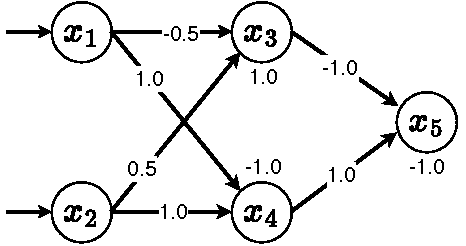
\includegraphics[width=0.5\linewidth]{figure/dnn.pdf}
    \caption{\label{fig:dnn} An FNN with ReLU.}
\end{figure}


\section{Types of Neural Networks}


\paragraph{Feed-Forward Network (FFN)} In an FFN information flows in one direction, from the input layer to hidden layers to the output layer (and thus no cycle).  

A fully connected feed-forward neural network (FNN), shown below, is an FFN where every neuron in a layer is connected to every neuron in the next layer.
\begin{center}
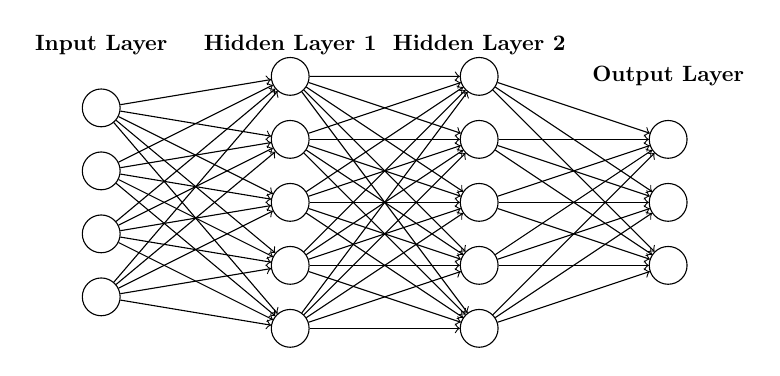
\begin{tikzpicture}[scale=0.8, transform shape]
% Input Layer
\node at (0,4) {\textbf{Input Layer}};
\foreach \x in {1,2,3,4} {
    \node[circle, draw=black, fill=white, minimum size=0.6cm] (I\x) at (0,4-\x) {};
}

% Hidden Layer 1
\node at (3,4) {\textbf{Hidden Layer 1}};
\foreach \x in {1,2,3,4,5} {
    \node[circle, draw=black, fill=white, minimum size=0.6cm] (H1\x) at (3,4.5-\x) {};
}

% Hidden Layer 2
\node at (6,4) {\textbf{Hidden Layer 2}};
\foreach \x in {1,2,3,4,5} {
    \node[circle, draw=black, fill=white, minimum size=0.6cm] (H2\x) at (6,4.5-\x) {};
}

% Output Layer
\node at (9,3.5) {\textbf{Output Layer}};
\foreach \x in {1,2,3} {
    \node[circle, draw=black, fill=white, minimum size=0.6cm] (O\x) at (9,3.5-\x) {};
}

% Connections
\foreach \i in {1,2,3,4}
    \foreach \j in {1,2,3,4,5}
        \draw[->] (I\i) -- (H1\j);

\foreach \i in {1,2,3,4,5}
    \foreach \j in {1,2,3,4,5}
        \draw[->] (H1\i) -- (H2\j);

\foreach \i in {1,2,3,4,5}
    \foreach \j in {1,2,3}
        \draw[->] (H2\i) -- (O\j);

\end{tikzpicture}
\end{center}





\paragraph{Convolutional Neural Networks (CNNs)} are a type of neural network that is often used in image recognition and classification.  CNNs consist of of neurons that have learnable weights and biases. Each neuron receives several inputs, takes a weighted sum over them, passes it through an activation function, and responds with an output.

\paragraph{Recurrent Neural Networks} Recurrent Neural Networks (RNNs) are a type of neural network that is often used in natural language processing and speech recognition. RNNs are designed to recognize patterns in sequences of data. RNNs have loops in them, allowing information to persist. This loop allows information to be passed from one step of the network to the next.

\paragraph{Residual Networks} Residual Networks (ResNets) are a type of neural network that is often used in image recognition and classification. ResNets introduce skip connections that allow the gradient to flow directly through the network, making it easier to train deep networks.

\section{Properties of Neural Networks}
Similar to software programs, neural networks have desirable properties to ensure the network behaves as expected. These could be specific to the applications modeled by the network, e.g., safety properties in a collision avoidance system or general properties that are desired by all networks, e.g., robustness to adversarial attacks. 


\paragraph{Robustness Properties}
\emph{Robustness}, a desirable property for all networks, ensures that small perturbations in the input data do not cause major changes in the output of the network. For example, if a few pixels in an image are changed, the network should still classify the image correctly. \emph{Adversarial attacks} are a common way to test the robustness of a neural network. In an adversarial attack, an attacker makes small changes to the input data to cause the network to misclassify the data.

\emph{Local} robustness refers to robustness of a neural network within a \emph{small neighborhood or region} of the input data. In contrast, \emph{global} robustness refers to robustness of a network across the \emph{entire input space}. Global robustness is harder to achieve than local robustness, as it requires the network to be robust to all possible inputs.

\paragraph{$\epsilon$-robustness} A neural network is $\epsilon$-robust if the difference between any two inputs $x$ and $x'$ is within a small range $\epsilon$, the output $f$ of the network does not change significantly (or remain the same), i.e., $\|x-x'\| \leq \epsilon \implies f(x) \approx f(x')$.




\paragraph{Safety Properties} Safety properties are specific to the application modeled by the network. For example, a safety property in a collision avoidance system might be that if the intruder is distant and significantly slower than us, then we stay below a certain threshold, i.e., $d_{intruder} > d_{threshold} \land v_{intruder} < v_{threshold} \implies v_{us} < v_{threshold}$.


\subsection{Challenges}

\paragraph{Formalization}


\paragraph{Expressiveness}




\chapter{Verification of Neural Networks}\label{sec:verification}
\paragraph{DNN Verification} Given a DNN \(N\) and a property $\phi$, the \emph{DNN verification problem} asks if $\phi$ is a valid property of $N$.
Typically, $\phi$ is a formula of the form $\phi_{in} \Rightarrow \phi_{out}$, where $\phi_{in}$ is a property over the inputs of $N$ and $\phi_{out}$ is a property over the outputs of $N$.
%This form of properties has been used to encode safety and security requirements of DNNs, e.g., safety specifications to avoid collision in unmanned aircraft~\cite{kochenderfer2012next} and \emph{adversarial robustness}~\cite{katz2017towards} properties desired by all DNNs, in which a small input perturbation does not cause major spikes in the DNN's outputs.
A DNN verifier attempts to find a \emph{counterexample} input to $N$ that satisfies $\phi_{in}$ but violates $\phi_{out}$.  If no such counterexample exists, $\phi$ is a valid property of $N$. Otherwise, $\phi$ is not valid and the counterexample can be used to retrain or debug the DNN~\cite{huang2017safety}.




% Verification tool such as Marabou and nnenum are then applied to the network to prove that the network is safe or identifier counterexample representing small input differences causing large output changes.


% \footnote{This is encoded as the differences of the inputs being within a certain small range  ($\phi_{in}$) implies the differences of the outputs still fall within a certain range in $\phi_{out}$)}.



\paragraph{Example} A valid property for the DNN in \autoref{fig:dnn} is that the output is $x_5 \le 0$ for any inputs $x_1 \in [-1,1], x_2\in[-2,2]$. An invalid property for this network is that $x_5 > 0$ for those similar inputs.
A counterexample showing this property violation is $\{x_1=-1, x_2=2\}$, from which the network evaluates to $x_5=-3.5$. Such properties can capture \emph{safety requirements} (e.g., a rule in an  collision avoidance system in~\cite{kochenderfer2012next,katz2017reluplex} is ``if the intruder is distant and significantly slower than us, then we stay below a certain threshold'') or \emph{local robustness}~\cite{katz2017towards} conditions (a form of adversarial robustness stating that small perturbations of a given input all yield the same output).


\section{Complexity}

\chapter{Search Algorithms}




\begin{algorithm}[t]
    \SetKwFor{Parfor}{parfor}{do}{endparfor}

    \SetKwInOut{Input}{input}
    \SetKwInOut{Output}{output}
    
    \SetKw{Break}{break}
    \SetKw{Continue}{continue}
    \SetKw{In}{in}
    
    \SetKwData{model}{model}
    \SetKwData{layer}{layer}
    \SetKwData{nextlayer}{layer$_{i+1}$}
    \SetKwData{prooftree}{proof}
    \SetKwData{leaf}{node}
    \SetKwData{status}{status}
    \SetKwData{minimum}{objval}
    \SetKwData{mynull}{null}
    
    \SetKwFunction{InputMILP}{AddInputConstrs}
    \SetKwFunction{GetUnstableNeurons}{GetUnstableNeurons}
    \SetKwFunction{PiecewiseLinearMILP}{AddConstrsPWL}
    \SetKwFunction{LinearMILP}{AddConstrsLinear}
    \SetKwFunction{Maximize}{Maximize}
    \SetKwFunction{Minimize}{Minimize}
    \SetKwFunction{Feasible}{CheckFeasibility}
    \SetKwFunction{Optimize}{Optimize}
    \SetKwFunction{isPiecewiseLinear}{isPiecewiseLinear}
    \SetKwFunction{CreateStabilizedMILP}{CreateStabilizedMILP}
    \SetKwFunction{GetLeafNodes}{GetLeafNodes}
    \SetKwFunction{AddConstrs}{AddConstrs}
    \SetKwFunction{RemoveConstrs}{RemoveConstrs}
    \SetKwFunction{AddObjective}{AddObjectives}
    \SetKwFunction{ShortenSplitConstrs}{ShortenSplitConstrs}
    \SetKwFunction{RemoveLeafNodes}{RemoveLeaves}
    \SetKwFunction{StoppingConditions}{StoppingConditions}
    \SetKwFunction{RepOK}{RepOK}
    \SetKwFunction{RaiseError}{RaiseError}

    \SetKwInOut{Input}{input}
    \SetKwInOut{Output}{output}
    \SetKw{Break}{break}
    \SetKw{Continue}{continue}
    \SetKwFunction{Backtrack}{Backtrack}
    \SetKwFunction{Select}{Select}
    \SetKwFunction{Decide}{Decide}
    \SetKwFunction{BCP}{BCP}
    \SetKwFunction{Deduce}{Deduce}
    \SetKwFunction{AnalyzeConflict}{AnalyzeConflict}
    \SetKwFunction{BooleanAbstraction}{BooleanAbstraction}
    \SetKwFunction{AddClause}{AddClause}
    \SetKwFunction{isTotal}{isTotal}
    \SetKwFunction{randomattack}{RandomAttack}
    \SetKwFunction{pgd}{PGDAttack}
    
    \SetKwFunction{DPLLT}{DPLLT}
    \SetKwFunction{isValid}{isValid}
    \SetKwFunction{isEmpty}{isEmpty}
    \SetKwFunction{LPSolver}{LPSolver}
    \SetKwFunction{Solve}{Solve}
    \SetKwFunction{FindLayerNodes}{FindLayerNodes}
    \SetKwFunction{TightenInputBounds}{TightenInputBounds}
    \SetKwFunction{Abstract}{Abstract}
    \SetKwFunction{Check}{Check}
    \SetKwFunction{Decide}{Decide}
    \SetKwFunction{Imply}{Imply}
    \SetKwFunction{Lower}{LowerBound}
    \SetKwFunction{Upper}{UpperBound}
    \SetKwFunction{GetInputBounds}{GetInputBounds}
    \SetKwFunction{GetInputs}{GetInputs}
    \SetKwFunction{GetNumInputs}{GetNumInputs}
    \SetKwFunction{CurrentConflictClause}{CurrentConflictClause}
    \SetKwFunction{StopCriterion}{StopCriterion}
    \SetKwFunction{LastAssignedLiteral}{LastLiteral}
    \SetKwFunction{LiteralToVariable}{LiteralToVariable}
    \SetKwFunction{Antecedent}{Antecedent}
    \SetKwFunction{BinRes}{BinRes}
    \SetKwFunction{BacktrackLevel}{BacktrackLevel}
    \SetKwFunction{AddClause}{AddClause}
    \SetKwFunction{ActivationStatus}{ActivationStatus}
    \SetKwFunction{Backjump}{Backjump}
    \SetKwFunction{EstimateBounds}{EstimateBounds}
    
    \SetKwData{problems}{ActPatterns}
    \SetKwData{implicationgraph}{igraph}
    \SetKwData{literal}{lit}
    \SetKwData{variable}{var}
    \SetKwData{antecedent}{ante}
    \SetKwData{conflict}{conflict}
    \SetKwData{none}{none}
    \SetKwData{layerid}{lid}
    \SetKwData{hiddenbounds}{hidden\_bounds}
    \SetKwData{layerbounds}{layer\_bounds}
    \SetKwData{inputs}{inputs}
    \SetKwData{inputbounds}{input\_bounds}
    \SetKwData{outputbounds}{output\_bounds}
    \SetKwData{infeasible}{INFEASIBLE}
    \SetKwData{unreachable}{UNREACHABLE}
    \SetKwData{maxinputs}{MAX\_NUM\_INPUT}
    \SetKwData{assignment}{$\sigma$}
    \SetKwData{dl}{dl}
    \SetKwData{lpmodel}{solver}
    \SetKwData{clauses}{clauses}
    \SetKwData{conflict}{conflict}
    \SetKwData{clause}{clause}
    \SetKwData{igraph}{igraph}
    \SetKwData{cex}{cex}
    \SetKwData{sat}{sat}
    \SetKwData{unsat}{unsat}
    \SetKwData{certified}{certified}
    \SetKwData{uncertified}{uncertified}
    \SetKwData{submodel}{sub\_model}
    
    \SetKwData{true}{true}
    \SetKwData{false}{false}
    \DontPrintSemicolon
    
    \SetKwFunction{Restart}{Restart}
    
    \SetKwData{counterexample}{cex}
    \SetKwData{conflictclause}{conflict\_clause}
    \SetKwData{isconflict}{is\_conflict}

    \footnotesize
    \DontPrintSemicolon
  
    \Input{DNN $\mathcal{N}$, property $\phi_{in} \Rightarrow \phi_{out}$}
    Output{($\unsat, \prooftree$)}
    \Output{($\unsat, \prooftree$) if property is valid, otherwise ($\sat, \counterexample$)}
    \BlankLine


    $\problems \leftarrow \{ \emptyset \}$ \tcp{initialize verification problems} 
    $\prooftree \gets \{ ~ \}$ \tcp{initialize proof tree}\label{line:prooftree}
    
    \While(\tcp*[h]{main loop}){$\problems$}{\label{line:dpllstart}
        % \tcp{$\sigma_i$ is the activation pattern of problem $i$-th}
        $\sigma_i \gets \Select(\problems)$ \tcp{process problem $i$-th}
        % \Parfor(\tcp*[h]{process in parallel}){$\sigma_i ~\In~ \problems$}{ \label{line:parfor}
            \If{\Deduce{$\mathcal{N}, \phi_{in}, \phi_{out}, \sigma_i$}}{\label{line:deduce}
                $(\counterexample, v_i) \leftarrow \Decide(\mathcal{N}, \phi_{in}, \phi_{out}, \sigma_i)$ \\ \label{line:decide}
                \If(\tcp*[h]{found a valid counter-example}){$\counterexample$}{
                    \Return{$(\sat, \counterexample)$} 
                }
                \tcp{create new activation patterns}
                $\problems \leftarrow \problems \cup \{ \sigma_i \land v_i ~;~ \sigma_i \land \overline{v_i} \}$ \;
            }
            \Else(\tcp*[h]{detect a conflict}){
                % $\clauses \leftarrow \clauses \cup \AnalyzeConflict(\igraph_i)$ \\ \label{line:analyze_conflict}
                $\prooftree \leftarrow \prooftree \cup \{ \sigma_i \}$ \tcp{build proof tree} \label{line:record_proof}
            }
        % }
        % \If(\tcp*[h]{no more problems}){$\isEmpty(\problems)$}{
        % }
        
    }\label{line:dpllend}
    \Return{$(\unsat, \prooftree)$}
    
    \caption{The \dd{} algorithm with proof generation.}\label{fig:alg}
\end{algorithm}

\autoref{fig:alg} shows \dd{}, a reference architecture~\cite{nakagawa2014consolidating} 
for modern DNN verifiers that we use to illustrate our observations.  
\dd{} takes as input a ReLU-based DNN $\mathcal{N}$ and a formulae $\phi_{in}\Rightarrow \phi_{out}$ representing the property of interest.

\dd{} iterates between two components: \texttt{Decide} (branching, \autoref{line:decide}), which decides (assigns) an activation status value for a neuron, and \texttt{Deduce} (bounding, \autoref{line:deduce}), which checks the feasibility of the current activation pattern. 
To add proof generation capability, \dd{} is instrumented with a proof tree (\texttt{proof}) variable (\autoref{line:prooftree}) to record these branching decisions. The proof is represented as a binary tree structure, where each node represents a neuron and its left and right edges represent its activation decision (active or inactive). %The proof tree is then used to generate a proof in the \nnproofformat{} format (\autoref{sec:proof-format}).




\begin{figure}[t]
    \begin{minipage}[b]{\linewidth}
        \centering
        \begin{minipage}[t]{0.48\textwidth}
            \centering  
            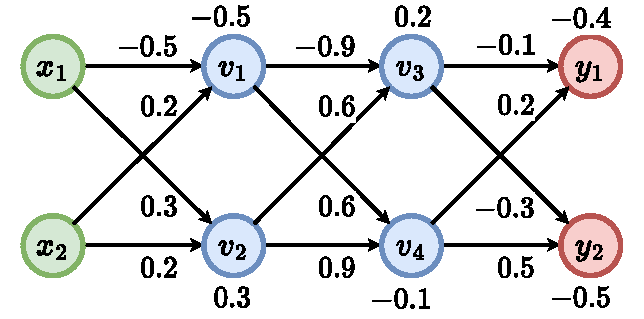
\includegraphics[width=\linewidth]{figure/proof_net.pdf}
            \caption*{(a)}
        \end{minipage}
        \begin{minipage}[t]{0.48\textwidth}
            \centering
            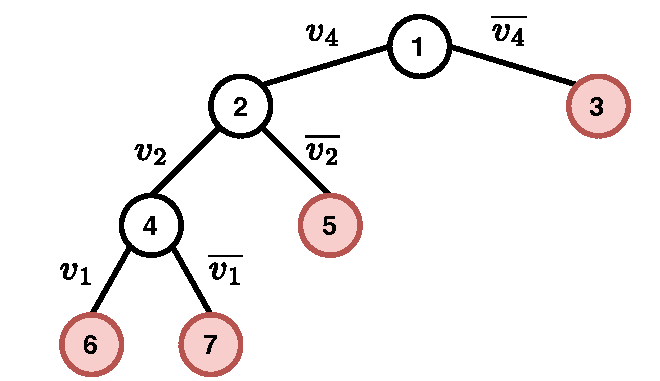
\includegraphics[width=\linewidth]{figure/proof_tree.pdf}
            \caption*{(b)}
        \end{minipage}
        \caption{(a) A simple DNN.  (b) A proof tree produced verifying the property $(x_1, x_2) \in [-2.0, 2.0] \times [-1.0, 1,0] \Rightarrow (y_1 > y_2)$.}
        \label{fig:example}
    \end{minipage}
\end{figure}
%White nodes correspond to branching nodes where \neuralsat{} makes decisions to split ReLU neurons.

\paragraph{Example} \autoref{fig:example}a illustrates a DNN and how \dd{} determines unsatisfiability (i.e., verifies the problem) and generates the unsat proof in \autoref{fig:example}b.

First, \dd{} initializes the activation pattern set \functiontextformat{ActPatterns} with an empty activation pattern $\emptyset$. Then \dd{} enters a loop (\autoref{line:dpllstart}-\autoref{line:dpllend}) to search for a satisfying assignment or a proof of unsatisfiability. In the first iteration, \dd{} selects the only available activation pattern $\emptyset \in \functiontextformat{ActPatterns}$. 
It calls \functiontextformat{Deduce} to check the feasibility of the problem based on the current activation pattern. \functiontextformat{Deduce} uses abstraction to approximate that from the input constraints the output values are feasible for the given network. 
Since \functiontextformat{Deduce} cannot decide infeasibility, \dd{} randomly selects a neuron to split (\functiontextformat{Decide}). Let us assume that it chooses $v_4$ to split, which essentially means the problem is split into two independent subproblems: one with $v_4$ active and the other with $v_4$ inactive.
\dd{} then adds $v_4$ and $\overline{v_4}$ to \functiontextformat{ActPatterns}.

In the second iteration, \dd{} has two subproblems (that can be processed in parallel). For the first subproblem with $v_4$, \functiontextformat{Deduce} cannot decide infeasibility, so it selects $v_2$ to split. It then conjoins $v_4$ with $v_2$ and then with $\overline{v_2}$ and adds both conjuncts to \texttt{ActPatterns}. 
For the second subproblem with $\overline{v_4}$ inactive, \functiontextformat{Deduce} determines that the problem is unsatisfiable and \dd{} saves the node $v_4$ to the proof tree, as node 3, to indicate one unsatisfiable pattern, i.e., whenever the network has $v_4$ being inactive, the problem is unsatisfiable.

In the third iteration, \dd{} has two subproblems for $v_4 \land v_2$ and $v_4 \land \overline{v_2}$. For the first subproblem, \functiontextformat{Deduce} cannot decide infeasibility, so it selects $v_1$ to split. It then conjoins $v_1$ and then $\overline{v_1}$ to the current activation pattern and adds them to \functiontextformat{ActPatterns}. For the second subproblem, \functiontextformat{Deduce} determines that the problem is unsatisfiable and \dd{} saves the node $v_4 \land \overline{v_2}$ to the proof tree, as node 5.

In the fourth iteration, \dd{} has two subproblems for $v_4 \land v_2 \land v_1$ and $v_4 \land v_2 \land \overline{v_1}$. Both subproblems are determined to be unsatisfiable, and \dd{} saves them to the proof tree as nodes 6 and 7, respectively.

Finally, \dd{} has an empty \texttt{ActPatterns}, stops the search, and returns \texttt{unsat} and the proof tree. 



\chapter{Constraint Solving}
\section{SMT}
\section{MILP}
\chapter{Abstraction}

\section{Interval}
\section{Zotope}
\section{Polytope}

\chapter{Popular Techniques and Tools}
\chapter{Verifying the Verifiers}
\chapter{Conclusion}

\bibliographystyle{abbrv}
\bibliography{ennv.bib}

\end{document}
